% ----------------------------------------------------------
\chapter{Revisão Bibliográfica}\label{cap:desenvolvimento}
% ----------------------------------------------------------
	Neste capítulo contextualizamos os objetos de estudo utilizados no trabalho iniciando por uma revisão teórica sobre a definição e diferentes classificações de aerossóis. Em seguida apresentamos referencial teórico sobre jato de baixos níveis com ênfase no fenômeno sul-americano, detalhando seus impactos no clima do continente e critérios de identificação.
% ----------------------------------------------------------
\section{Aerossóis}
% ----------------------------------------------------------

	Define-se o conceito de aerossol por uma coleção de partículas, sólidas ou líquidas, suspensas em um gás, com dimensões que variam entre alguns micrômetros até dezenas de nanômetros. No contexto da meteorologia, se atribui o termo "aerossol" apenas às partículas suspensas, sem levar em conta o gás atmosférico \autocite{boucher2015,seinfeld2006}. Seus impactos são diversos, pois interagem de forma direta com as radiações terrestre e solar através da absorção e espalhamento das mesmas, e também indiretamente ao atuarem como núcleos de condensação de nuvens, o que atribui aos mesmos um papel importante não só no balanço de radiação do planeta, mas também no sistema hidrológico e elétrico terrestre \autocite{carslaw2022a}.  Adicionalmente, é pertinente vincular a discussão à uma perspectiva de saúde humana, uma vez que a poluição do ar é o segundo maior fator de risco para morte em escala global \autocite{stateofglobalair2025}.
	
	No que compete à classificação, existem diversas propostas para sistematizar as diferentes populações de aerossóis na atmosfera. As abordagens mais usadas se baseiam na composição química das partículas, no seu processo de formação e no seu local de origem \autocite{boucher2015}.
	

% ----------------------------------------------------------
\subsection{Processo de Formação}
% ----------------------------------------------------------
	Considera-se um aerossol primário quando o material é emitido na atmosfera com forma, composição química e tamanho relativamente definidos, não havendo necessidade de interações físico-químicas para que o mesmo atinja seu estágio final. Como exemplos temos o sea spray, proveniente do atrito entre ventos e a superfície do oceano, partículas de poeira suspensas a partir de solo exposto às intempéries, além de fuligem criada por combustão incompleta de material orgânico \autocite{boucher2015}. 
	Aerossóis secundários são formados a partir de gases já suspensos na atmosfera, denominados precursores segundo \textcite{boucher2015}, que acabam por se tornarem aerossóis através do processo de nucleação. De acordo com \textcite{seinfeld2006}, esse fenômeno é parte da mudança de fase em processos termodinâmicos e faz referência ao fato de que a alteração de estado da matéria não ocorre de forma homogênea e nem instantânea, mas sim em agrupamentos que vão aumentando ao longo do tempo. No contexto de aerossóis secundários, conforme adotado por \textcite{boucher2015}, é de interesse simplificar o termo ”nucleação” ao agrupamento das moléculas sem a presença de um núcleo ou superfícies distintas que servirão de alicerce para o processo. Exemplos de precursores de aerossóis são dióxido de enxofre (SO2), amônia (NH3), Compostos Orgânicos Voláteis (COV), Óxidos de Nitrogênio (NOx) e Sulfeto de Dimetila (DMS) \autocite{carslaw2022a}. Um esquema conceitual da emissão, interação com a atmosfera e fim do ciclo de vida de aerossóis, tanto primários quanto secundários, e sua relação de distribuição de tamanhos ao longo desses processos é apresentado na Figura \ref{fig:process}.
	
	

\begin{figure}[htb]
	\begin{center}
		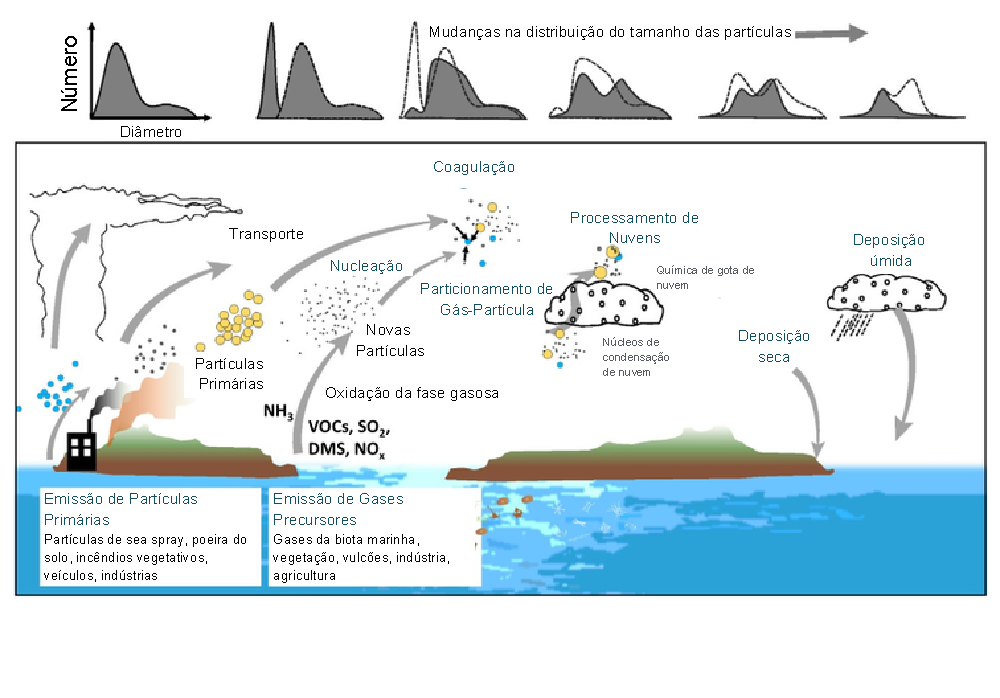
\includegraphics[trim=0cm 1.7cm 0cm 0cm, clip]{images/figura1.pdf}

	\end{center}
	\caption{Processos de transformação química e microfísica de aerossóis na atmosfera. A evolução aproximada da distribuição de tamanho das partículas é mostrada na linha superior correspondente ao processo na figura principal \autocite{carslaw2022a}.}
	\label{fig:process}
\end{figure}

\subsection{Composição Química}
		Adicionalmente, é vantajoso classificar aerossóis por sua composição química quando o intuito é entender de forma mais detalhada os impactos desses materiais na atmosfera. A partir dessa organização é possível atribuir maior ou menor grau de protagonismo em processos de absorção e espalhamento de radiação e no processo de formação de nuvens. Por exemplo, aerossóis do tipo Black Carbon\footnote{A literatura usa o termo Black Carbon fazendo alusão à alta eficiência desse aerossol em absorver radiação solar e ao aspecto escurecido de fumaça de combustão \autocite{petzold2013}.}, com sua estrutura física exemplificada na Figura \ref{fig:bc_struc}, são originais de processos incompletos de queima de material orgânico e possuem um perfil muito higroscópico, o que os torna mais propensos a agirem como Núcleos de Condensação de Nuvens. Aerossóis Inorgânicos também são higroscópicos, porém contribuem pouco para o balanço radiativo do planeta \autocite{boucher2015}.
	\begin{figure}[htb]
		\begin{center}
			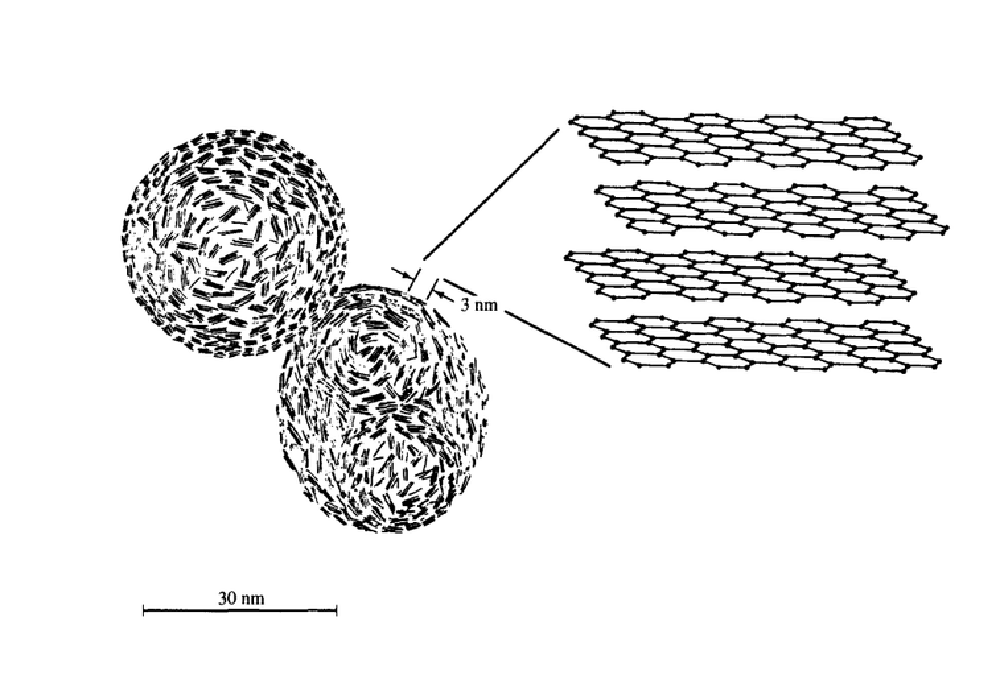
\includegraphics{images/figura2.pdf}
		\end{center}
		\caption{Esquema microestrutural de uma partícula de fuligem \autocite{seinfeld2006}}
		\label{fig:bc_struc}
	\end{figure}

\subsection{Distribuição Espacial e Temporal}
	Outra abordagem conveniente para sistematizar aerossóis se dá pelo local onde são produzidos. \textcite{boucher2015} faz distinção entre fontes naturais e antropogênicas. No que diz respeito às fontes naturais, temos oceanos, desertos, erupções vulcânicas e vegetação como fontes emissoras. Quanto às antropogênicas, leva-se em conta a ação humana na produção de aerossóis, como a queima de combustíveis fósseis e biocombustíveis, atividades tanto industriais como domésticas, além de queimadas de vegetação oriundas de ação humana. 
	
	\begin{figure}[htb]
		\begin{center}
			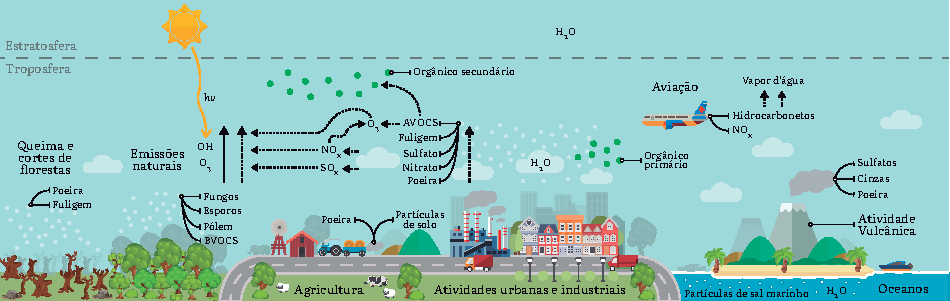
\includegraphics{images/figura3.pdf}
		\end{center}
		\caption{Principais fontes primárias e secundárias de aerossol e seu processamento na atmosfera a partir da interação entre as diversas fontes e também com a radiação solar \autocite{nascimento2021}.}
		\label{fig:nasc}
	\end{figure}

	
	Além de fontes, \textcite{boucher2015} também define o conceito de sumidouro de aerossóis, responsáveis pela deposição dessas partículas. As duas formas principais de finalizar o ciclo de vida de um aerossol são a deposição seca, que ocorre quando a partícula entra em contato com a superfície do planeta e a deposição úmida, quando a mesma é usada como núcleo de condensação para precipitação. A Figura \ref{fig:nasc} esquematiza as fontes de aerossol no sistema terrestre e suas interações com a atmosfera. 
	Por último, o que define o tempo de vida de um grupo de aerossóis na atmosfera além dos locais de gênese e deposição, é a forma com que ambos interagem com o mecanismo de transporte responsável por deslocar essas partículas de um ponto a outro.

\subsection{Distribuição de Tamanho de Partículas e Propriedades Ópticas}

	Para estudos de qualidade do ar, é comum que a nomenclatura mude de aerossóis para termos como poluentes e material particulado, com esse último englobando principalmente partículas suspensas no ar com até 1, 2.5 e 10 micrômetros em diâmetro, conforme indicado na Figura \ref{fig:uepa}. A partir dessas classificações são elaboradas legislações que visam estabelecer limites para a quantidade de materiais particulados que podem estar presentes em um local com riscos mínimos à saúde humana \autocite{usepa2019}.
	
	\begin{figure}[htb]
		\begin{center}
			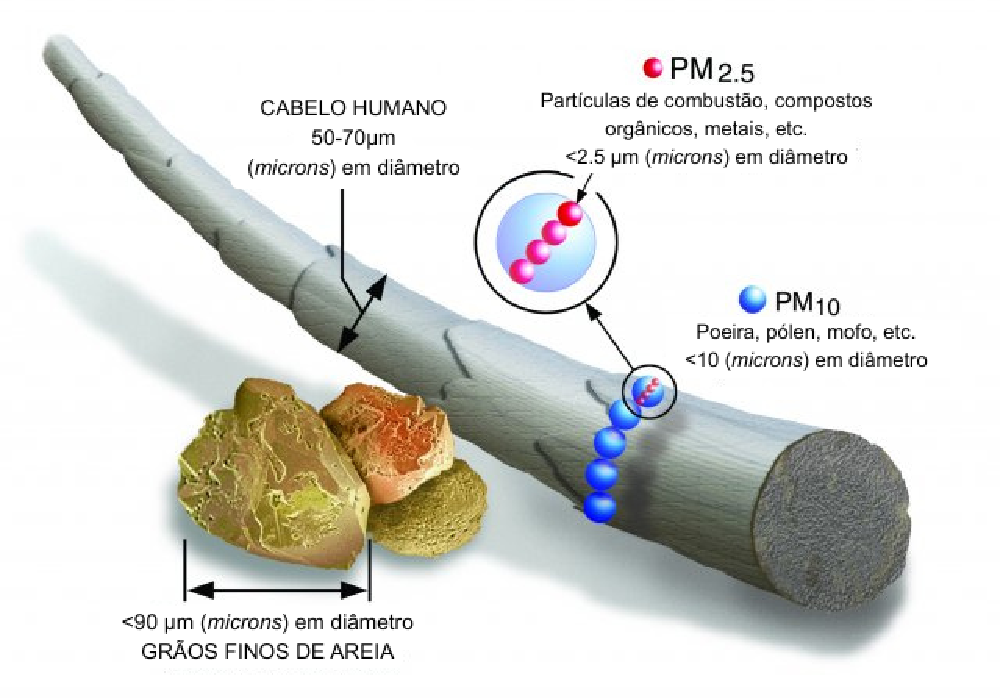
\includegraphics{images/figura4.pdf}
		\end{center}
		\caption{Figura 4: Esquema de comparação de tamanhos de MP10 e MP2.5 \autocite{usepa2019}.}
		\label{fig:uepa}
	\end{figure}  
	  
	Outra forma comum de analisar dados dessa natureza é através da profundidade óptica estimada através de satélites, onde o ponto de grade diz respeito à quantidade da partícula em questão presente em toda aquela coluna de ar, dessa forma, não é possível discretizar a concentração em níveis de altura \autocite{boucher2015}. Para os estudos de profundidade óptica e outras análises de sensoriamento, a Figura \ref{fig:distribuicao_classica} apresenta a distribuição de tamanho com mais detalhe tanto para aerossóis primários quanto secundários.
	
	\begin{figure}[htb]
	\begin{center}
		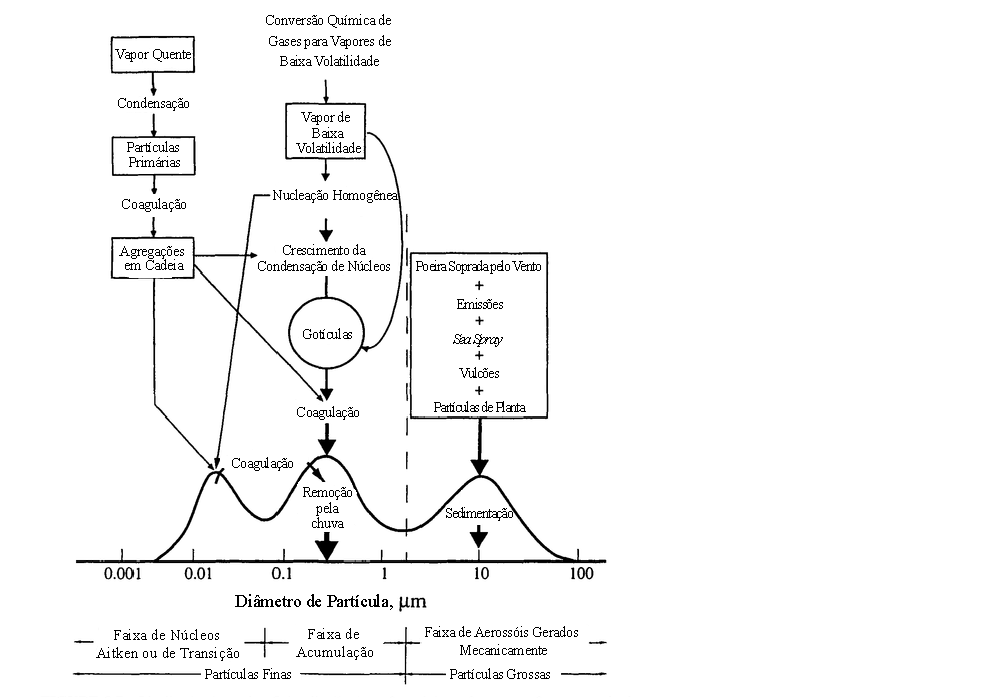
\includegraphics[trim=0cm 0cm 5cm 0cm, clip]{images/figura5.pdf}
	\end{center}
	\caption{Esquema idealizado da distribuição de área de superfície de partícula de um aerossol atmosférico, adaptado de \textcite{whitby1976}. Os principais modos, fontes e formação/remoção de partículas estão indicados.}
	\label{fig:distribuicao_classica}
	\end{figure}
	
	
	
\section{Jato de Baixos Níveis}
	Segundo \textcite{lin2007}, o Jato de Baixos Níveis (JBN) é um fenômeno de mesoescala, com distribuição horizontal na escala de milhares de quilômetros e temporal de alguns dias, composto de corrente de ar que se desloca com altas velocidades próximo à superfície terrestre, entre 2 e 3 km de altura. Sua importância para a meteorologia se dá por ser um mecanismo de transporte de temperatura e umidade, além de possuir dinâmicas muito específicas influenciadas pela orografia e ter uma relação intrínseca com a ocorrência de outros fenômenos atmosféricos de mesoescala. Os exemplos mais significativos são o JBN das grandes planícies nos Estados Unidos e o JBN da América do Sul, mas também existem registros da ocorrência desse mesmo fenômeno em diversos outros lugares. Em primeira instância, a caracterização do JBN se deu pelo Critério de \textcite{bonner1968}, onde o sistema se configura através de:
	\begin{itemize}
		\item Ventos meridionais iguais ou superiores a 12 $ms^{-1}$ no nível de 850 hPa;
		\item Cisalhamento vertical do vento de no mínimo 6 $ms^{-1}$ entre os níveis de 700 e 850 hPa;
		\item Componente meridional do vento maior em extensão que a componente zonal; \autocite{marengo2009}. 
	\end{itemize}
	
\section{Jato de Baixos Níveis da América do Sul}
	Ainda de acordo com \autocite{marengo2009}, o Jato de Baixos Níveis da América do Sul, comumente referido por South American Low-Level Jet (SALLJ), é um fenômeno recorrente na América do Sul caracterizado por um fluxo intenso de ventos a leste da cordilheira dos Andes, conforme indicado na Figura \ref{fig:sallj}.  Os estudos com relação ao tópico iniciaram na década de 1980 e encontraram avanços significativos com as tecnologias de reanálise de dados e modelagem numérica da atmosfera, sendo possível identificar que o mesmo nem sempre ocorre de forma homogênea ou contínua ao longo da América do Sul \autocite{jones2019}.  Por conta da floresta amazônica e sua alta injeção de umidade na atmosfera, \autocite{herdies2002} aponta o SALLJ como parte de um mecanismo bimodal de redistribuição tanto de umidade quanto de calor partindo da região norte da AS em direção às regiões centrais e sul do Brasil, atuando em conjunto com a Zona de Convergência do Atlântico Sul (ZCAS) ao longo da estação chuvosa (meses de verão), o que favorece a ocorrência de eventos de precipitação intensos com grande impacto nas regiões sul e sudeste do país. Adicionalmente, o transporte de umidade contribui em outros momentos na formação e manutenção de Complexos Convectivos de Mesoescala e sistemas frontais comuns na região \autocite{reboita2015}. 
	
	Quanto aos pormenores de sua classificação, \autocite{montini2019} argumenta que o critério previamente utilizado, por ter sido elaborado com valores empíricos obtidos nas Grandes Planícies da América do Norte, apresenta vieses na identificação de eventos de ocorrência do SALLJ, uma vez que o perfil de ventos na América do Sul apresenta uma variabilidade sazonal muito distinta quando comparada com os dados obtidos por \autocite{bonner1968} e adaptados por \autocite{marengo2009}. Em sua análise do fenômeno por uma perspectiva climatológica, a autora atualiza o critério de Bonner/Marengo se baseando em  percentis climatológicos do perfil de ventos e fluxos de umidade elaborados com reanálises e sondagens. A partir disso, os critérios são:
	
	\begin{itemize}
		\item Velocidade do vento em 850 hPa excedendo o percentil 75\% para a época do ano em questão;
		\item Cisalhamento vertical do vento entre 850 e 700 hPa também excedendo o percentil citado anteriormente;
		\item Direção do vento em 850 hPa entre 292.5° e 45°; \autocite{montini2019}.
	\end{itemize}
	
	\autocite{montini2019} também conclui que o SAALJ ocorre em quantidade muito maior do que o considerado pelos antigos parâmetros ao longo do ano, com as máximas de velocidade do vento permanecendo nos meses de inverno.
	
	\begin{figure}[htb]
		\begin{center}
			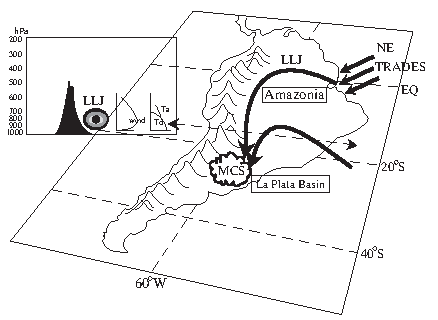
\includegraphics{images/figura6.pdf}
		\end{center}
		\caption{Modelo conceitual descrevendo o JBN da América do Sul a leste dos Andes \autocite{marengo2004}.}
		\label{fig:sallj}
	\end{figure}
	
	
	Outro resultado interessante proveniente dos avanços da tecnologia na área de sensoriamento remoto dentro do estudo dos Jatos é a possibilidade de replicar o conceito de mecanismo de transporte para outros componentes da atmosfera, como é o caso do transporte de aerossóis através de rios atmosféricos \autocite{chakraborty2022}. Mais especificamente, \autocite{forgioni2025} utilizam do SALLJ para caracterizar o transporte em longa distância de aerossóis provenientes de queimadas na Amazônia para os estados de São Paulo e Rio Grande do Sul em setembro de 2024. 

\section{Bloqueios Atmosféricos}
\label{sec:bloqueio}
	
	De acordo com \textcite{holton2012introduction}, o escoamento de ar em latitudes médias possui um sentido predominantemente zonal e de oeste em médios e altos níveis, como resultado do equilíbrio geostrófico, entre as forças defletora e Coriolis e a força Gradiente de Pressão. Essa característica da atmosfera é responsável pelo deslocamento espacial de diferentes fenômenos atmosféricos ao longo do tempo. Porém, num contexto de bloqueio atmosférico, a componente meridional do escoamento é alongada por conta da combinação de centros de alta e baixa pressão estacionários (de no mínimo seis dias). Como consequência, a intensidade, extensão e duração desses sistemas sinóticos são alteradas drasticamente \autocite{ambrizzi2009bloqueios}.
	
	
	No Hemisfério Sul, em especial, \textcite{mendes2008blocking} destaca como impacto de Bloqueios no Sul do Brasil a alteração nos regimes precipitação, como o impedimento do avanço de sistemas frontais, os quais influenciam na remoção de aerossóis da atmosfera através do processo de deposição úmida: os aerossóis são utilizados como núcleos de condensação para nuvens (\textit{in-cloud scavenging}) e são arrastados para a superfície através dos fluxos de ar provenientes da precipitação (\textit{below-cloud scavenging}) \autocite{boucher2015}.   
	Como formas de identificação, \textcite{rex1950effect} foi o primeiro a mapear as características comuns aos padrões de bloqueios, com \textcite{vanloon1956blocking} refinando a pesquisa para o Hemisfério Sul:
	\begin{itemize}
		\item O deslocamento do sistema de bloqueio, dados pelo movimento do centro de alta, não deve exceder 25° de longitude em 45°S durante todo seu período;
		\item O centro do anticiclone de bloqueio deve estar pelo menos 10° de latitude mais ao sul do cinturão de altas pressões subtropicais;
		\item O bloqueio deve durar pelo menos seis dias.
	\end{itemize}
	
 
	
	As diferentes possibilidades de configuração de circulação que podem ser encontradas em bloqueios atmosféricos estão representadas na Figura \ref{fig:block}.
	\begin{figure}[htb]
		\begin{center}
			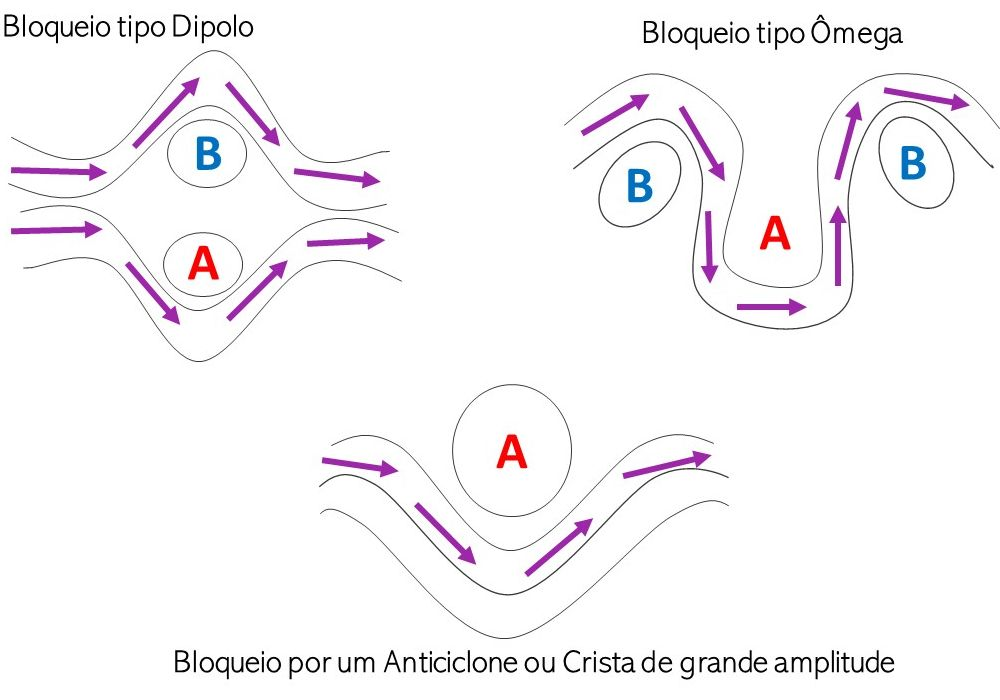
\includegraphics[width=\textwidth]{images/tiposdebloqueio.jpg}
		\end{center}
		\caption{Os três tipos de padrões de bloqueios e as alterações sofridas pelos Jatos de Altos Níveis (setas roxas). \autocite{bueno2019bloqueios}.}
		\label{fig:block}
	\end{figure}